% =====================================================================
% Beamer 슬라이드: 다회검정과 다층모형
%   Gelman, Hill, & Yajima (2012)
% Compile with: xelatex slides.tex
% =====================================================================
\documentclass[10pt,aspectratio=169]{beamer}

\usepackage{fontspec}
\setmainfont[BoldFont={Noto Sans KR Bold}]{Noto Sans KR}
\setsansfont[BoldFont={Noto Sans KR Bold}]{Noto Sans KR}
\setmonofont{Latin Modern Mono}

\usepackage{amsmath,amssymb,bm}
\usepackage{graphicx}
\usepackage{booktabs}
\usepackage{xcolor}
\usetheme{metropolis}
\IfFileExists{beamerthemeMetropolis.sty}{}{\usetheme{default}}

\setbeamertemplate{navigation symbols}{}
\setbeamertemplate{frametitle}[default][center]
\setbeamercolor{frametitle}{bg=blue!15,fg=blue!50!black}

\newcommand{\Normal}{\mathcal{N}}
\newcommand{\E}{\mathbb{E}}

\title{다회검정 문제와 다층모형}
\subtitle{Why We (Usually) Don't Have to Worry About Multiple Comparisons \\
         \footnotesize Gelman, Hill, \& Yajima (2012)}
\author{}
\date{}

\begin{document}

% ---------------------------------------------------------------------
\begin{frame}\titlepage\end{frame}

% ---------------------------------------------------------------------
\begin{frame}{용어 안내}
본 강의에서는 \alert{\textbf{다회검정 (multiple comparisons; 多回檢定)}} 을 표준 용어로 사용합니다.

\bigskip
한국 통계학회에서 통용되는 \alert{``다중비교''}도 동일한 의미로 사용됩니다.
\bigskip

\begin{block}{왜 ``다회검정''인가?}
문제의 본질: \emph{하나의 데이터에 검정을 \textbf{여러 번 반복}하기 때문에 누적 오류율이 부풀어 오른다}.
``다중(多重)''의 ``겹쳐 누적된'' 뉘앙스는 부정확. ``다회(多回)''의 ``여러 차례''가 본질을 더 정확히 포착.\\
다만 ``다중비교''/``다중검정''이 학계 표준이므로 두 표현 모두에 익숙해질 것.
\end{block}
\end{frame}

% =====================================================================
\section{문제 제기}

\begin{frame}{문제: 다회검정은 항상 보정해야 할까?}
교육·정책 평가에서 매일 나오는 질문:
\begin{itemize}
  \item 8개 학교에서 진행한 코칭 프로그램, 어느 학교에서 효과?
  \item 50개 주의 성적 순위, 어느 주가 의미 있게 다른가?
  \item 1{,}000명 교사의 효과 추정치, 어떤 교사가 특별히 좋은가?
\end{itemize}
\bigskip

전통적 빈도주의 답: \alert{p-value를 보정}하라 --- Bonferroni, FDR, Sidak, \ldots
\bigskip

Gelman 등의 답: \alert{문제 자체를 다시 생각}하자.
\end{frame}

\begin{frame}{이 강의의 결론을 미리 보면}
\begin{block}{핵심 주장}
\begin{enumerate}
  \item Type 1 error 패러다임은 사회과학에서 적절한 출발점이 아니다.
        (``진짜 효과 = 0''이 거의 항상 거짓.)
  \item 진짜 위험은 \alert{Type S}와 \alert{Type M} error.
  \item 다층(hierarchical) 모형은 다회검정 보정을 \alert{모델 안에 내재화}한다.
        Ad-hoc한 p-value 조작 불필요.
\end{enumerate}
\end{block}
\end{frame}

% =====================================================================
\section{빈도주의 관점}

\begin{frame}{IHDP 예제 (8개 사이트)}
저체중·미숙아에게 가정방문/양질의 보육 서비스 제공.
각 사이트별 처치 효과 $\delta_j$를 추정.

\bigskip
고전적 모형:
\[
  y_i = \sum_{j=1}^{8}\bigl(\gamma_j S_i^j + \delta_j S_i^j P_i\bigr) + \varepsilon_i
\]
$\varepsilon_i \sim \Normal(0,\sigma^2)$.

\bigskip
각 사이트에 대해 $H_0^j: \delta_j = 0$ 을 \emph{독립적으로} 검정.
\end{frame}

\begin{frame}{Family-Wise Error Rate가 부풀어 오른다}
$\alpha = 0.05$로 8번 검정:
\[ \Pr(\text{적어도 한 번 잘못 기각}) = 1 - 0.95^8 \approx 0.34 \]

\bigskip
\textbf{Bonferroni}: 임계값을 $\alpha / k = 0.05/8 = 0.00625$로 낮춤 \\
신뢰구간을 $z_{0.99688} \approx 2.73$ 으로 \emph{넓힘} (1.96 대비)
\end{frame}

\begin{frame}{IHDP 시뮬레이션 결과}
\begin{center}
  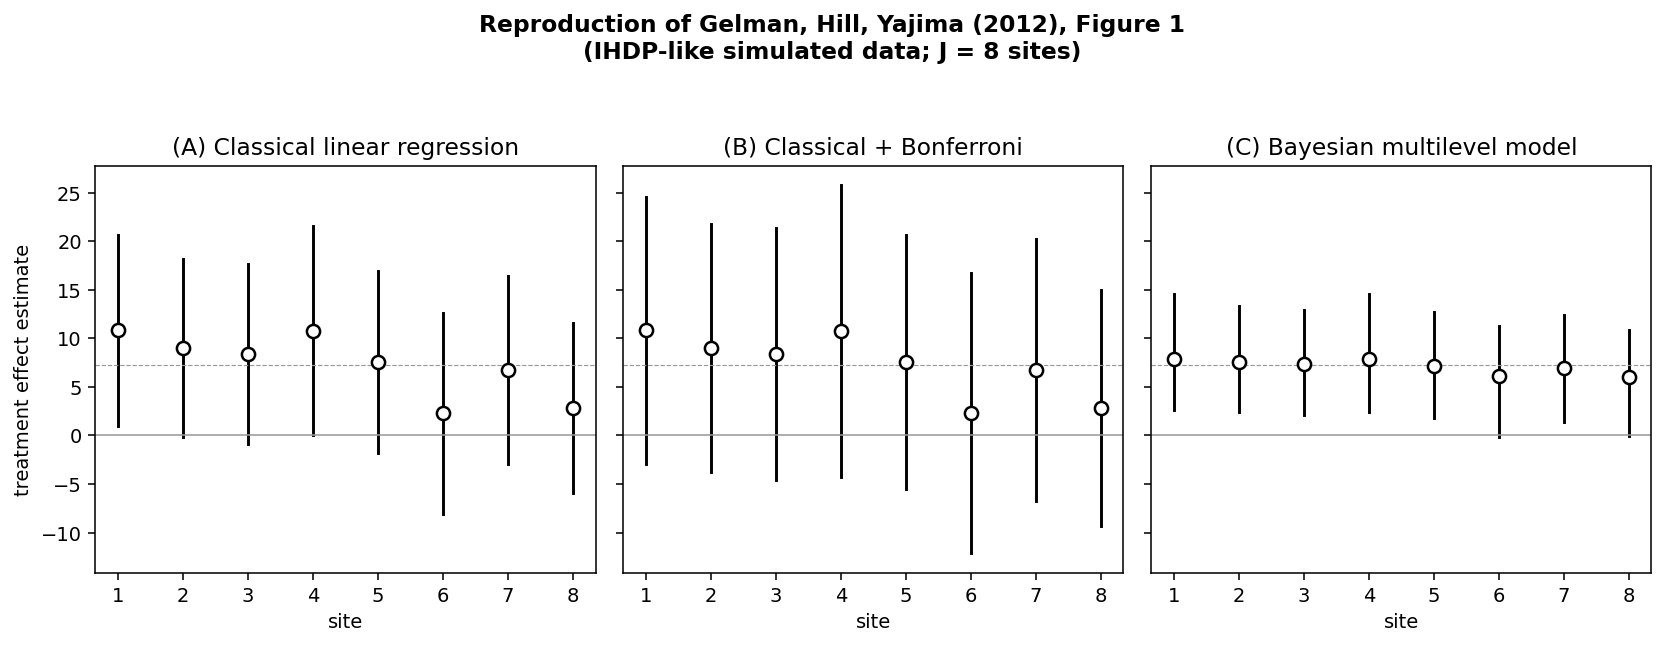
\includegraphics[width=\linewidth]{../figures/fig_ihdp_three_panels.png}
\end{center}
\footnotesize
(A) 사이트별 OLS는 잡음으로 흩어진다.\\
(B) Bonferroni는 폭만 넓히고 점은 그대로.\\
(C) 다층모형은 점 자체를 평균 부근으로 끌어당긴다.
\end{frame}

% =====================================================================
\section{Type S \& Type M error}

\begin{frame}{Type 1/2 대신: Type S와 Type M}
\begin{itemize}
  \item \alert{Type S} (sign): 진짜 효과의 \emph{부호}를 거꾸로 추정.
  \item \alert{Type M} (magnitude): 유의한 추정치가 진짜 효과보다 \emph{훨씬 크다}.
\end{itemize}
\bigskip
저전력 (큰 SE) 일수록 ``유의''에 살아남은 결과는 더 극단적이 된다.
\begin{center}
  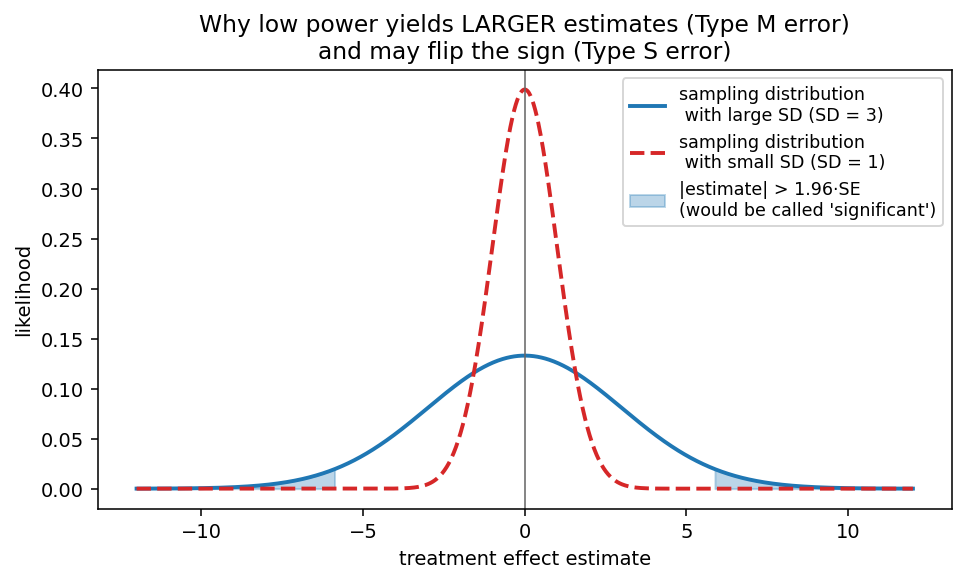
\includegraphics[width=0.6\linewidth]{../figures/fig_type_sm_intuition.png}
\end{center}
\end{frame}

\begin{frame}{시뮬레이션: 진짜 효과 = 2}
\begin{center}
  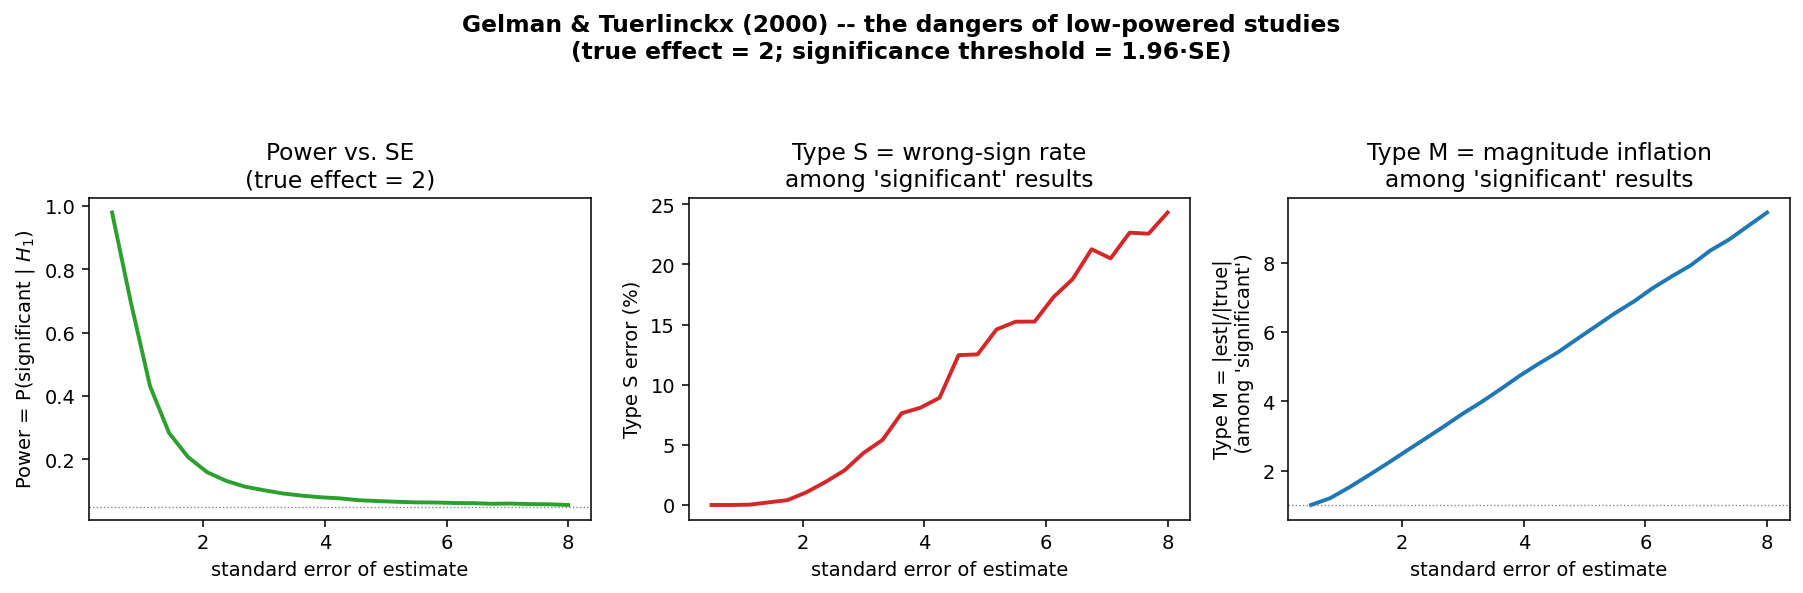
\includegraphics[width=\linewidth]{../figures/fig_type_sm_simulation.png}
\end{center}
\footnotesize
SE가 커질수록 power는 떨어지지만 \emph{유의 결과의 부호 오류율}과 \emph{과대 추정 비율}이 폭증.\\
\textbf{Bonferroni는 사실상 SE를 더 크게 만든다} → Type S/M을 \emph{악화}.
\end{frame}

\begin{frame}{빈도주의가 자주 하는 실수}
\begin{enumerate}
  \item ``유의하면 효과가 있는 것, 유의하지 않으면 효과가 없는 것이다.''\\
        \alert{틀린 명제.}
  \item ``Bonferroni를 적용했으니 안전하다.''\\
        \alert{Type 1만 통제. Type 2/S/M은 \emph{악화}.}
  \item ``8개 사이트는 다 다르니 각자 따로 분석하자.''\\
        \alert{다층모형은 사이트가 얼마나 다른지를 데이터에서 결정.}
\end{enumerate}
\end{frame}

% =====================================================================
\section{다층모형의 정의와 직관}

\begin{frame}{다층(Hierarchical) 모형}
\[
\begin{aligned}
  y_i      &\sim \Normal(\gamma_{j[i]} + \delta_{j[i]} P_i, \sigma_y^2) \\
  \gamma_j &\sim \Normal(\mu_\gamma, \sigma_\gamma^2) \\
  \delta_j &\sim \alert{\Normal(\mu_\delta, \sigma_\delta^2)}
\end{aligned}
\]
\bigskip
\alert{이 한 줄}이 모든 것을 바꾼다:
\begin{itemize}
  \item $\delta_j$들이 \emph{공통 분포}에서 나왔다고 본다.
  \item $\sigma_\delta \to 0$:  사이트는 사실상 같음 (complete pooling)
  \item $\sigma_\delta \to \infty$: 사이트는 완전히 다름 (no pooling)
  \item $\sigma_\delta$ 자체를 \emph{데이터에서 추정} $\Rightarrow$ partial pooling
\end{itemize}
\end{frame}

\begin{frame}{Shrinkage의 대수}
가장 간단한 정규-정규 모형:
\[ \bar y_j \mid \theta_j \sim \Normal(\theta_j, \sigma_{\bar y}^2),\quad \theta_j \sim \Normal(\mu, \sigma_\theta^2). \]

\bigskip
사후 평균:
\[ \E[\theta_j \mid \bar y_j] = w_j \bar y_j + (1-w_j)\mu, \quad w_j = \tfrac{\sigma_\theta^2}{\sigma_\theta^2 + \sigma_{\bar y}^2} \]

\bigskip
$w_j$가 ``개별 정보를 얼마나 믿을지'' 결정.\\
잡음이 크면 ($\sigma_{\bar y}$ 큼) $\to w_j$ 작음 $\to$ 공통 평균 쪽으로 강하게 끌어당김.
\end{frame}

\begin{frame}{z-score의 shrinkage (논문 Fig.~4)}
\begin{center}
  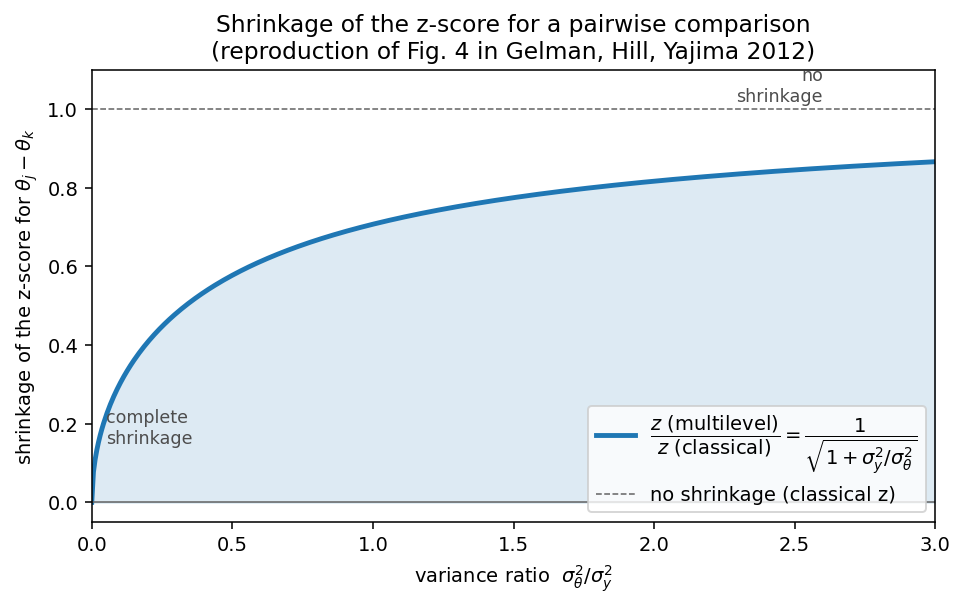
\includegraphics[width=0.65\linewidth]{../figures/fig_shrinkage_zscore.png}
\end{center}
\footnotesize
두 그룹 차이의 z-score는 항상 다음 인자로 감소:
\[ z_{\mathrm{MLM}} = z_{\mathrm{classical}} \cdot \frac{1}{\sqrt{1 + \sigma_{\bar y}^2/\sigma_\theta^2}} \]
\textbf{데이터-주도 다회검정 보정}이 자동으로 일어남.
\end{frame}

% =====================================================================
\section{예제 1: Eight Schools}

\begin{frame}{Eight Schools (Rubin 1981) -- 실제 데이터}
SAT-Verbal 코칭 효과 실험 (뉴저지 8개 고등학교):

\begin{center}\small
\begin{tabular}{ccc cc}
\toprule
School & $y_j$ & $\sigma_j$ & Bayes M & Bayes SD \\
\midrule
A & 28 & 15 & 11 & 8 \\
B &  8 & 10 &  7 & 6 \\
C & -3 & 16 &  6 & 8 \\
D &  7 & 11 &  7 & 7 \\
E & -1 &  9 &  5 & 6 \\
F &  1 & 11 &  6 & 7 \\
G & 18 & 10 & 10 & 7 \\
H & 12 & 18 &  8 & 8 \\
\bottomrule
\end{tabular}
\end{center}
\footnotesize
(원 논문 Table~1.)
\end{frame}

\begin{frame}{같은 데이터, 세 가지 시각}
\begin{center}
  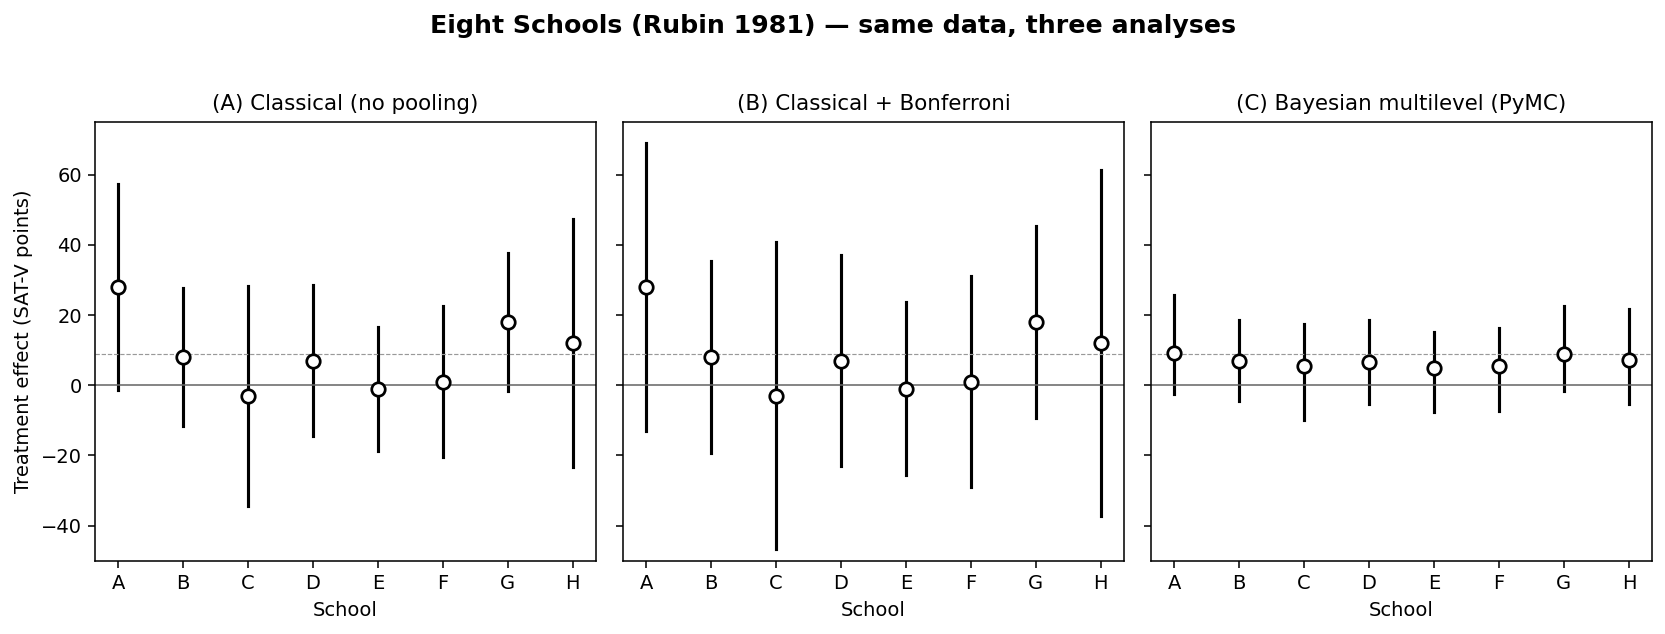
\includegraphics[width=\linewidth]{../figures/fig_eight_schools_compare.png}
\end{center}
\footnotesize
(A) raw 95\% CI, (B) Bonferroni, (C) Stan 다층모형.\\
사후 평균이 A=11, C=6으로 \emph{서로 가까워졌다}.
\end{frame}

\begin{frame}{Shrinkage가 일어나는 모습}
\begin{center}
  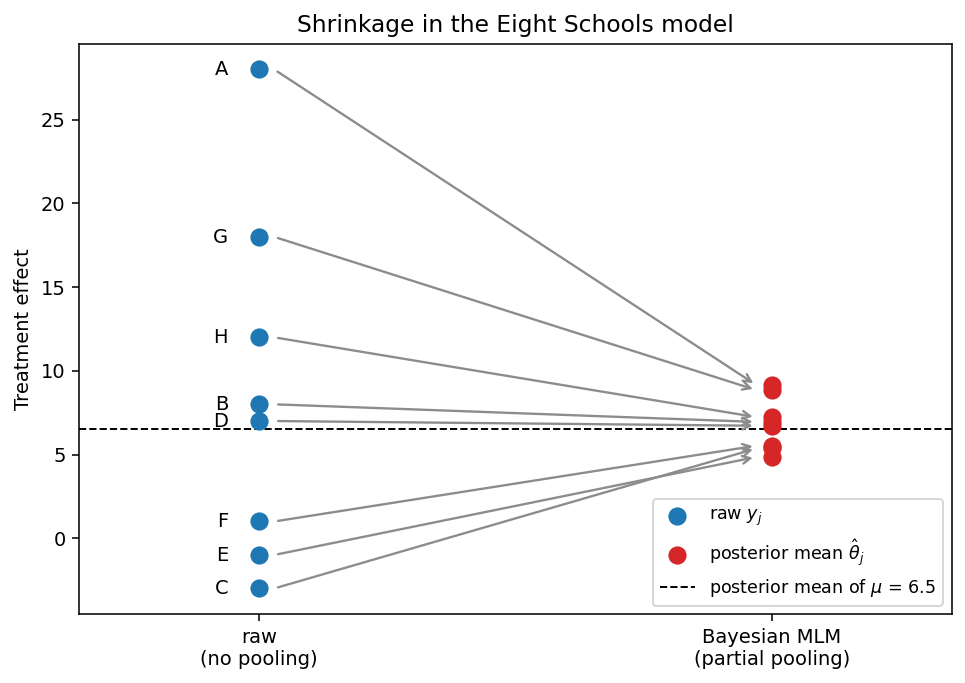
\includegraphics[width=0.65\linewidth]{../figures/fig_eight_schools_shrinkage.png}
\end{center}
\footnotesize
극단값 (A=28, G=18)이 가장 많이 끌려간다.
\end{frame}

\begin{frame}{왜 강한 shrinkage? -- $\tau$의 사후분포}
\begin{center}
  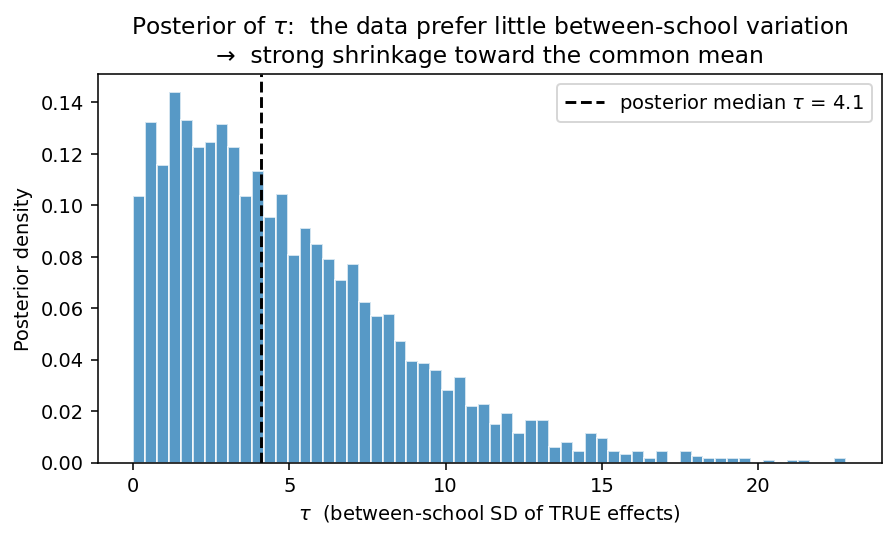
\includegraphics[width=0.65\linewidth]{../figures/fig_eight_schools_tau_posterior.png}
\end{center}
\footnotesize
$\tau$의 사후 질량이 0 부근에 집중되어 있음.\\
$\Rightarrow$ 데이터가 ``학교들의 진짜 효과는 별로 안 다르다''라고 말함.
\end{frame}

% =====================================================================
\section{구현: Stan + NumPyro}

\begin{frame}[fragile]{본 강의의 MCMC 도구}
\textbf{주력 (primary):} \alert{Stan / cmdstanpy}
\begin{itemize}
  \item 베이지안 모형링의 사실상 표준
  \item 풍부한 진단/요약 도구 (Rhat, ESS, divergence check, ...)
  \item Stan 문법은 모형 정의가 매우 명시적
\end{itemize}
\bigskip
\textbf{보조 (auxiliary):} NumPyro (JAX 기반)
\begin{itemize}
  \item C++ 툴체인 없이 순수 파이썬 환경에서 작동
  \item JIT 컴파일로 빠른 NUTS, GPU/TPU 활용 용이
  \item Stan과 동일한 NUTS 알고리즘
\end{itemize}
\bigskip
두 도구의 결과는 (충분한 sample size에서) 사실상 일치.
\end{frame}

\begin{frame}[fragile]{Stan 모형 (Eight Schools)}
\scriptsize
\begin{verbatim}
data {
  int<lower=1> J;
  vector[J] y;
  vector<lower=0>[J] sigma;
}
parameters {
  real mu;
  real<lower=0> tau;
  vector[J] eta;
}
transformed parameters {
  vector[J] theta = mu + tau * eta;
}
model {
  mu  ~ normal(0, 10);
  tau ~ normal(0, 10);   // half-normal
  eta ~ std_normal();
  y   ~ normal(theta, sigma);
}
\end{verbatim}
\end{frame}

\begin{frame}[fragile]{NumPyro 모형 (같은 Eight Schools)}
\scriptsize
\begin{verbatim}
def eight_schools_model(sigma, y=None):
    mu  = numpyro.sample("mu",  dist.Normal(0., 10.))
    tau = numpyro.sample("tau", dist.HalfNormal(10.))
    with numpyro.plate("school", J):
        eta   = numpyro.sample("eta", dist.Normal(0., 1.))
        theta = numpyro.deterministic("theta", mu + tau*eta)
        numpyro.sample("y", dist.Normal(theta, sigma), obs=y)

kernel = NUTS(eight_schools_model, target_accept_prob=0.95)
mcmc   = MCMC(kernel, num_warmup=1000, num_samples=2000, num_chains=4)
mcmc.run(rng_key, sigma, y=y)
\end{verbatim}
같은 모형, 같은 알고리즘 (NUTS), 같은 결과.
\end{frame}

% =====================================================================
\section{예제 2: IHDP 시뮬레이션}

\begin{frame}{IHDP 시뮬레이션 (8개 사이트, 사이트당 80명)}
참 효과: 평균 8.0, SD 1.2 (사이트 간 변동 작음).
\begin{center}
  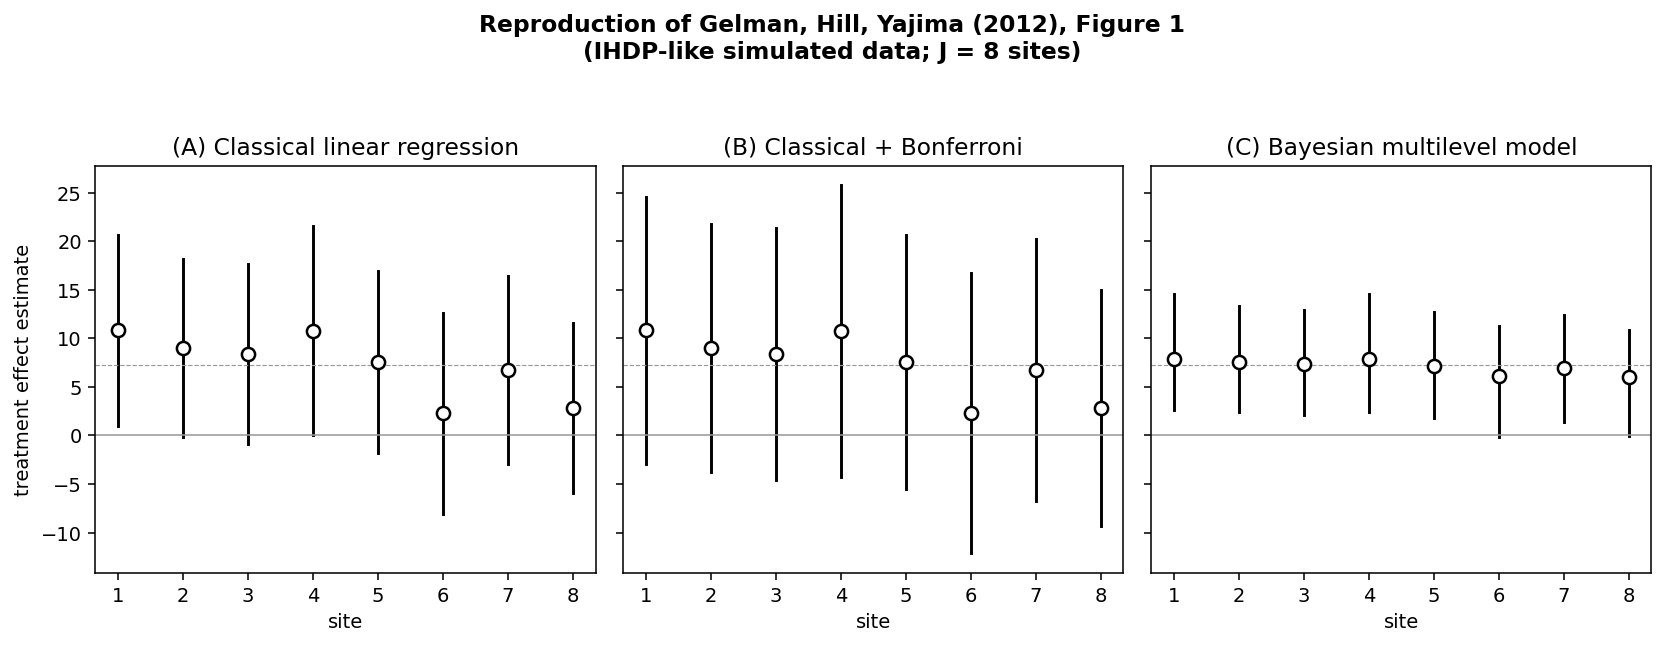
\includegraphics[width=\linewidth]{../figures/fig_ihdp_three_panels.png}
\end{center}
\footnotesize
다층모형 (Stan) 이 ``작은 OLS 추정치는 잡음일 가능성''을 자동 반영하여 평균 부근으로 끌어당김.
\end{frame}

\begin{frame}[fragile]{IHDP Stan 모형}
\scriptsize
\begin{verbatim}
parameters {
  real mu_gamma, mu_delta;
  real<lower=0> sigma_gamma, sigma_delta, sigma_y;
  vector[J] gamma_raw, delta_raw;
}
transformed parameters {
  vector[J] gamma = mu_gamma + sigma_gamma * gamma_raw;
  vector[J] delta = mu_delta + sigma_delta * delta_raw;
}
model {
  // weak half-normal priors on the sigmas
  gamma_raw ~ std_normal();
  delta_raw ~ std_normal();
  vector[N] mu_i;
  for (i in 1:N) mu_i[i] = gamma[site[i]] + delta[site[i]] * P[i];
  y ~ normal(mu_i, sigma_y);
}
\end{verbatim}
\end{frame}

% =====================================================================
\section{결론}

\begin{frame}{핵심 메시지}
\begin{block}{Gelman, Hill, Yajima (2012)}
\begin{itemize}
  \item 다회검정은 본질적으로 \alert{모형이 부족해서} 생긴다.
  \item Bonferroni/FDR은 신뢰구간을 \emph{넓혀} Type 1을 통제하지만,
        그 대가로 Type 2/S/M을 모두 \emph{악화}.
  \item 다층모형은 추정치 자체를 \emph{끌어당겨} 같은 목표를 달성하면서
        효과의 부호와 크기에 대한 \alert{더 신뢰할 만한} 추론을 준다.
  \item 게다가 점추정의 MSE는 OLS보다 더 작다 (\textbf{Stein paradox}).
\end{itemize}
\end{block}
\bigskip
\textbf{실무 권고:} 그룹 비교가 있는 모든 분석에 다층모형을 \emph{기본}으로 고려.
\end{frame}

\begin{frame}{학생에게 강조할 점 (요약)}
\begin{enumerate}
  \item \alert{``유의''와 ``효과 있음''은 같지 않다}. SE를 항상 함께 보고.
  \item \alert{저전력 + 유의 = 과대 추정 + 부호 오류 위험}.
  \item \alert{Bonferroni는 만능 보장이 아니다}. 진짜 효과를 못 보게 만들 수 있다.
  \item \alert{exchangeable 그룹은 항상 다층 우선}.
  \item \alert{$\tau$의 사후분포를 항상 확인}. 거기에 ``보정 강도''가 들어 있다.
  \item \alert{Stan을 우선 사용, NumPyro는 보완}. 두 도구 모두 익숙해질 것.
\end{enumerate}
\end{frame}

\begin{frame}{참고문헌}
\footnotesize
\begin{itemize}
\item Gelman, Hill, Yajima (2012). \emph{J.~Research on Educational Effectiveness}, 5: 189--211.
\item Rubin (1981). Estimation in parallel randomized experiments. \emph{J.~Educational Statistics}.
\item Gelman \& Tuerlinckx (2000). Type S error rates. \emph{Computational Statistics}.
\item Gelman (2006). Prior distributions for variance parameters in hierarchical models. \emph{Bayesian Analysis}.
\item Gelman \& Hill (2007). \emph{Data Analysis Using Regression and Multilevel/Hierarchical Models}.
\item Carpenter et al. (2017). Stan: A probabilistic programming language. \emph{JSS}, 76(1).
\item Phan, Pradhan, \& Jankowiak (2019). NumPyro. arXiv:1912.11554.
\end{itemize}
\end{frame}

\begin{frame}{질문 환영합니다}
\vfill
\begin{center}{\Huge 감사합니다}\end{center}
\vfill
\end{frame}

\end{document}
